%versi 3 (18-12-2016)
\chapter{Pengujian Terhadap Kode Program Sederhana}
\label{lamp:A}

\section{Kode Program}
\label{kodeProgram:A}
\lstinputlisting[language=Java, caption=OperasiMatematikaInterface.java]{./Lampiran/OperasiMatematikaInterface.java}
\lstinputlisting[language=Java, caption=Pembagian.java]{./Lampiran/Pembagian.java}
\lstinputlisting[language=Java, caption=Pengurangan.java]{./Lampiran/Pengurangan.java}
\lstinputlisting[language=Java, caption=Perkalian.java]{./Lampiran/Perkalian.java}
\lstinputlisting[language=Java, caption=Pertambahan.java]{./Lampiran/Pertambahan.java}
\section{Hasil Latex}
\label{hasilLatex:A}
\lstinputlisting[language=TeX, caption=operasimatematika.tex, label={operasimatematika}]{./Lampiran/operasimatematika.tex}
\section{Hasil PDF}
\label{hasilPDF:A}
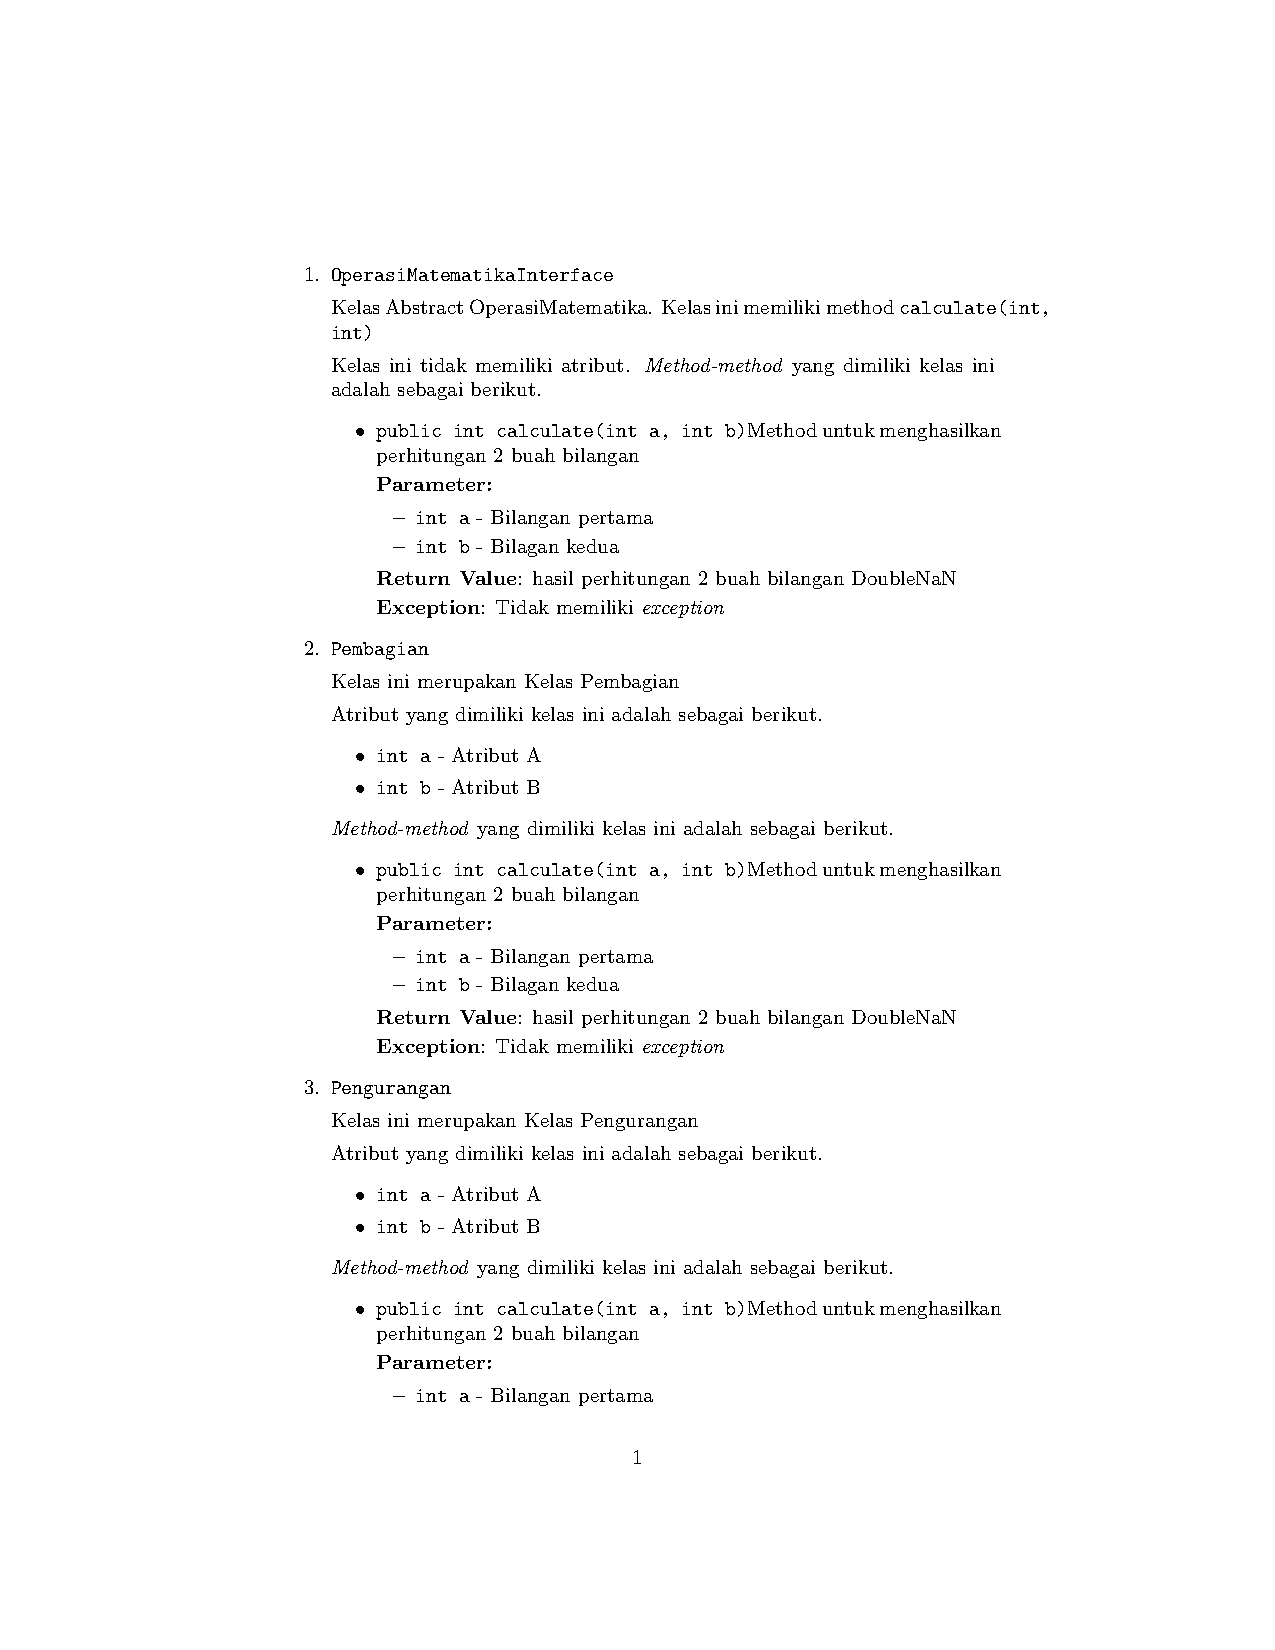
\includepdf[page=1]{./Lampiran/operasimatematika.pdf}
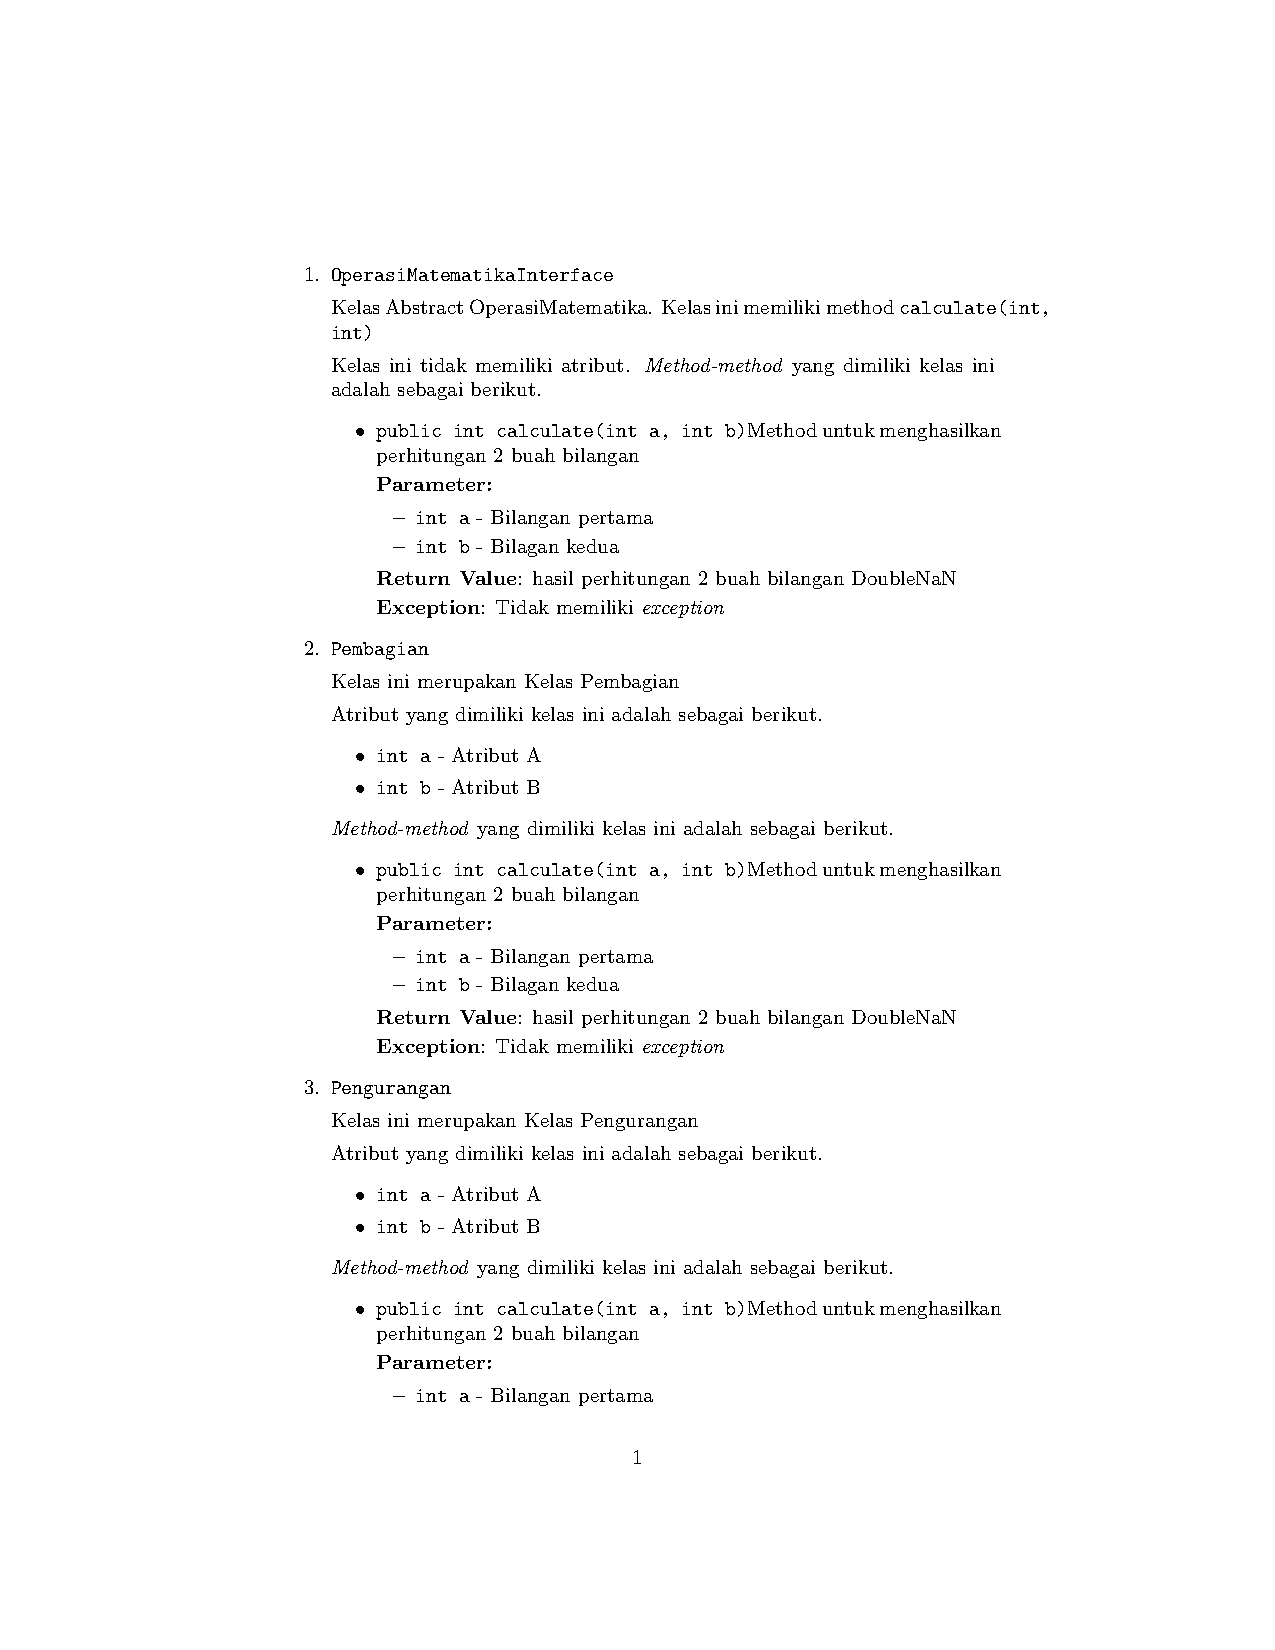
\includepdf[page=2,pagecommand={\null\vfill\captionof{figure}{operasimatematika.pdf}}]{./Lampiran/operasimatematika.pdf}










